\documentclass{standalone}
\usepackage{../../../../preamble_formulas}

\begin{document}

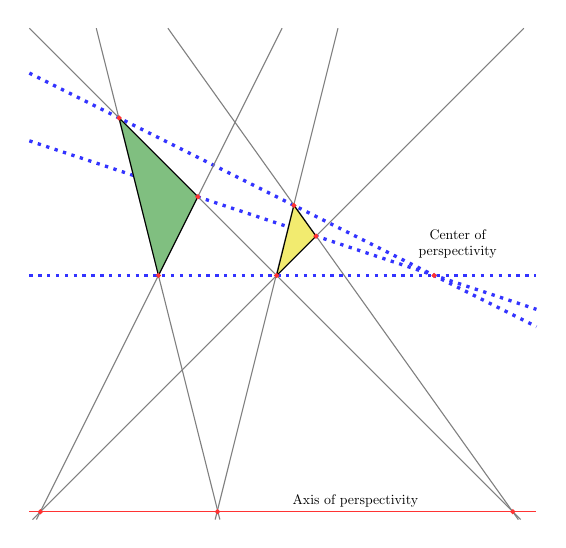
\begin{tikzpicture}
    %%% LINES
    \draw[color=red!80, thin] (-2.14,-3) -- (4.29,-3);
    \draw[color=blue!80, dotted, very thick] (-2.14,0) -- (4.3,0);
    \draw[color=blue!80, dotted, very thick] (-2.14,1.71) -- (4.3,-0.43);
    \draw[color=blue!80, dotted, very thick] (-2.14,2.57) -- (4.3,-0.65);
    \draw[color=gray, thin] (-2.05,-3.1) -- (1.07,3.14);
    \draw[color=gray, thin] (-2.1,-3.1) -- (4.14,3.14);
    \draw[color=gray, thin] (0.28,-3.1) -- (-1.29,3.14);
    \draw[color=gray, thin] (0.22,-3.1) -- (1.78,3.14);
    \draw[color=gray, thin] (4.07,-3.1) -- (-0.38,3.14);
    \draw[color=gray, thin] (4.1,-3.1) -- (-2.14,3.14);

    %%% TRIANGLES
    \filldraw[fill=black!50!green!50, thin] (-0.5,0) -- (0,1) -- (-1,2) -- cycle;
    \filldraw[fill=black!10!yellow!60, thin] (1,0) -- (1.5,0.5) -- (1.22,0.89) -- cycle;

    %%% POINTS
    %% TRIANGLES
    \filldraw[red!80] (-0.5,0) circle (0.7pt);
    \filldraw[red!80] (0,1) circle (0.7pt);
    \filldraw[red!80] (-1,2) circle (0.7pt);
    \filldraw[red!80] (1,0) circle (0.7pt);
    \filldraw[red!80] (1.5,0.5) circle (0.7pt);
    \filldraw[red!80] (1.22,0.89) circle (0.7pt);

    %% INTERSECTIONS
    \filldraw[red!80] (3,0) circle (0.7pt);
    \filldraw[red!80] (-2,-3) circle (0.7pt);
    \filldraw[red!80] (0.25,-3) circle (0.7pt);
    \filldraw[red!80] (4,-3) circle (0.7pt);

    %%% WORDS
    \node[scale=0.5,align=center] at (3.3,0.4) {Center of\\perspectivity};
    \node[scale=0.5,align=center] at (2,-2.87) {Axis of perspectivity};
\end{tikzpicture}

\end{document}